\chapter{绪\hspace{6pt}论}

\section{课题研究背景及意义}
合成孔径雷达(Synthetic Aperture Radar, SAR)是一种对地探测的主动式微波成像技术,通常通过搭载在飞机或卫星上来实现对地物目标的测量。相比于光学传感器,SAR系统不受天气条件、云层、光照等影响,能够实现全天时、全天候的成像,即使在恶劣天气条件下也能保持较高的成像质量\citing{皮亦鸣2007合成孔径雷达成像原理}。极化SAR在SAR的基础上,通过发射、接收不同极化方式的电磁波信号,实现对地物目标散射信息的探测。相比于基础的SAR系统,极化SAR具有更丰富的散射特征,蕴含更多的目标信息。目前,由于极化SAR的多极化特性,极化SAR技术已经成为合成孔径雷达技术中不可或缺的重要分支。在极化SAR的众多应用中,极化SAR图像解译工作已经成为其中最重要的研究方向之一,其目的是快速、准确地实现地物目标的分类识别,在军事目标探测、城市规划、灾害估计等多个军事民事领域已经得到了广泛应用\citing{pramudya2019estimation,gao2018ship}。

在解读极化SAR数据方面,极化SAR图像分类技术扮演着至关重要的角色。其核心在于特征提取和目标分类方法等技术的实施。可靠的地物目标分类结果依赖于合理且有效的特征提取工程和目标分类方法,才能充分体现出极化SAR复杂探测数据的重要价值。由于极化SAR的多极化成像特性,极化SAR数据中蕴含了丰富的目标散射信息,这些信息的应用则依赖于高效的极化特征表达技术。极化特征的准确表述构成了极化SAR分析的基础,并且是整个解译过程中至关重要的环节,对最终的分类结果具有重要的影响。利用合理的特征表示,能够使分类模型更加快速、准确的迭代到最优参数,取得优秀的分类结果;反之,不合理的特征表示即便是使用更加复杂的分类器模型,也很难达到出色的分类结果。极化SAR图像的目标分类也属于解译的关键步骤,其本质是为极化SAR图像中的每一个像素赋予准确的类别。目标分类算法的核心目标是建立一种非线性的判定机制,该机制能够根据样本的相似性特征将其划分到相应的类别中,分类器的设计关键就在于其有效区分同类和异类地物目标。

% 近年来,尽管极化SAR系统成像能力方面取得了持续进步与显著发展,但其图像解译技术方面发展却相对滞后,这也导致了极化SAR系统在实际工程中应用受到限制。随着极化SAR成像系统分辨率的不断提升,虽然为地物目标带来更加丰富的细节信息,但也为极化SAR图像数据解读研究带来了新的问题与挑战。首先,随着极化SAR图像特征表征技术的研究发展,涌现了越来越多的极化特征,这些特征从不同的角度对目标散射特征进行描述,如何有效整合并应用这些多元化的极化特征参数,以提升地物目标特征表示的准确性和完备性,成为极化SAR图像解译中的难点。其次,随着极化SAR成像技术的突破,获取到的极化SAR数据集呈现爆炸性增长趋势,但是标记这些数据集依赖专业知识,需要较大的人工成本和精确的标注技术,由于人工标记错误、自动标记技术精度不足等因素导致的错误标记样本问题给极化SAR图像解译带来巨大的困难\citing{tu2020robust,uhlmann2013integrating,liu2016large},如何在混杂有标签噪声的数据集中实现高准确率的分类结果也成为极化SAR图像解译中的新挑战。具体体现在以下两个方面:

近年来,尽管极化SAR系统成像能力方面取得了持续进步与显著发展,但其图像解译技术方面发展却相对滞后,这种不平衡的状况限制了极化SAR系统在实际工程中的广泛应用。尽管极化SAR成像系统分辨率的不断提升与获取到的极化SAR数据量显著增长为图像解译工作带来了积极作用,但同时也引入了新的困难与挑战。具体而言,体现在:

(1)极化SAR图像表现出高分辨率趋势,带来更为详尽的地物特征信息。目前,对极化SAR数据特征工程研究不断深入,极化特征提取方法日渐增多,这些方法从不同的角度对地物目标的散射特性进行描述。然而,当前大多数的极化SAR图像分类算法仅仅采用了单一类型的极化特征。复杂的空间场景具有更复杂的几何结构和散射特性。单一类型的极化特征无法全面地描述目标的细节信息,无法对目标信息进行全面概括。同时,不同类型的极化特征间可能存在较强的相关性与冗余性,且固定的极化特征表示方式无法在所有类型的地物目标和图像中取得满意的结果\citing{zhang2014fully,刘高峰2014极化,1017062722.nh,1021744178.nh}。如何有效整合并应用这些多元化的极化特征参数,以提升地物目标特征表示的准确性和完备性,成为极化SAR图像解译中的难点。

(2)极化SAR技术不断发展,极化SAR数据集数量呈现爆发式增长。对极化SAR数据集的标注工作依赖专业知识或自动标注技术,由于极化SAR的复杂成像特性,标注工作中不可避免地由于人工错误标记、自动标注技术精度不足等问题出现错误标记的样本。错误标记样本的信息会对分类器的分类规则形成不同程度的影响,导致分类准确率的下降\citing{tu2020robust,uhlmann2013integrating,liu2016large}。如何在混杂有噪声样本的数据集下实现高准确率的分类结果是当前极化SAR图像解译领域的研究难点。

针对上述问题,本文基于深度学习方法优势,首先研究极化SAR多类型极化特征有效信息挖掘方法,旨在降低多类型极化特征信息冗余,为目标分类任务提供高质量的极化特征表示。在此基础上,进一步研究标签噪声下鲁棒性的极化SAR目标分类方法,实现混杂标签噪声数据集中可靠分类,提升极化SAR系统的实用性。

\section{国内外相关研究现状}
极化SAR图像目标分类技术包含两个核心环节,即极化特征表示和分类器设计,本文内容围绕极化特征的表示方法和分类器的设计方法展开。因此,本节将对以上两个关键技术进行现状分析。

\subsection{极化SAR特征表示}
由于极化SAR的多极化、多通道的成像机制,极化SAR图像中蕴含了丰富的目标散射信息。将极化SAR原始散射数据转化为直观易懂且具有实用价值的地理信息是一项极具挑战的任务,这依赖于准确的极化特征表示方式。

% 极化SAR数据中隐含了大量的目标极化散射信息,而这些信息的挖掘与利用极度依赖于准确的极化特征表示方式。在极化SAR图像解译工作中,极化特征表示方法扮演着至关重要的基础角色。

现有的大多数极化SAR数据特征表示方法都是以像素为最基本的处理单元,依赖于每个单独像素点的固有特性实现特征提取与分类。根据表征目标属性意义差异,现有极化特征可以分为以下三类:
% 通常来说,常见的极化特征表示方法有对观测数据进行简算数运算构造的特征、基于极化目标分解理论的目标分解特征以及图像空间纹理特征等。

% (1)对观测数据进行算数运算构造的特征
(1)基于观测数据的物理特征

极化SAR图像的观测数据包括极化散射矩阵、多视处理后的相干矩阵和协方差矩阵等。这类特征利用简单的四则运算或组合变换对观测数据进行信息表示,主要有反射率、反射强度、幅度、相位等。Rignot等人\citing{rignot1992unsupervised}率先提出通过对极化协方差矩阵个元素取对数来实现极化SAR图像分割;Pierce等人\citing{pierce1994knowledge}结合了极化散射矩阵和专家系统的知识集成技术,开展了对极化SAR图像分类研究;Kong等人\citing{1988Identification}提出了采用极化散射矩阵中各通道的比例关系作为分类指标,用于极化SAR图像分类任务;Lee等人\citing{964970}运用散射矩阵计算得到相位差异信息,并结合最大似然算法对图像分类;Ding等人\citing{1017062722.nh}提取了散射矩阵和相干矩阵的元素,组合形成特征向量,用于分类研究。

基于观测数据的物理特征虽易于获取且直观明了,但是表征信息相对浅显,未能深入解释地物目标内部具体的物理散射机制。这一类特征因为简便而被广泛使用,但是在提供深层次物理信息方面存在一定的局限性。

% Rignot等人\citing{rignot1992unsupervised}提出了使用极化协方差矩阵中的各个元素的对数来实现极化SAR图像的分割;Pierce等人\citing{pierce1994knowledge}结合极化散射矩阵和专家系统展开了对极化SAR图像的分类研究;Kong等人\citing{1988Identification}提出了利用极化散射矩阵每个通道的强度之比来进行极化SAR图像分类研究工作;Lee等人\citing{964970}使用散射矩阵计算出相位差,结合最大似然分类器进行分类;Ding等人\citing{1017062722.nh}从散射矩阵和相干矩阵中的各个元素组成特征向量,用于分类研究。基于观测数据算数运算构造的极化特征属于最基本的极化特征表示方式,简单易得,但是缺少了对地物目标的具体物理散射机制的深层解释。

(2)基于目标分解的散射特征

极化目标分解理论通过从物理散射意义层面对极化SAR数据进行约束,来反映地物目标确切物理意义的散射特性,是极化SAR数据利用中最为经典且至关重要的理论之一。1970年,Huynen首次提出了目标分解理论\citing{huynen1970phenomenological,huynen1990stokes},为极化SAR特征表示方法研究奠定了理论基础。极化目标分解方法是使用多个散射基将极化SAR数据分解为多个具有不同物理意义的矩阵分类加权和的形式。根据处理的数据差异,可以分为极化相干分解和极化非相干分解两种形式,分别用于处理极化散射矩阵和极化相干矩阵或协方差矩阵。

极化相干分解针对散射矩阵数据,从物理层面进行约束,利用不同的基向量将散射矩阵分解为不同物理意义的矩阵分量加权和。典型的极化相干分解方法包括Pauli分解\citing{cloude1996review}、Krogager分解\citing{krogager1990new}以及Cameron分解\citing{cameron1990feature}等。Pauli分解将散射矩阵分解为分别对应单次散射、方位角为0°和45°的二次散射效应的综合;Krogager分解则是将散射矩阵分解为球形散射、二面角散射和螺旋型散射三类散射机制的组合形态;Cameron分解在Pauli分解基础上进行拓展,提出以经过旋转调整后的最大散射分量作为主要分解特征。

% 相干分解要求目标具有稳定的散射性质和相干的散射波,适用于没有噪声的环境,对于存在一个主要目标的场景效果优越,能够准确地表达地物目标的物理散射特性。

极化非相干分解方法针对多视矩阵数据,将其分解为多个反映确切物理意义的参数加权和的形式。典型的非相干分解技术包括Cloude分解\citing{cloude1997entropy}、Freeman分解\citing{freeman1998three}以及Holm分解\citing{holm1988radar}等。Cloude分解立足于矩阵特征值理论,通过分析相关矩阵的最大特征值来推测地物目标的散射特性类别,并且引入了一系列具有重要意义的极化散射特征参数,如散射熵、各项异性指数和平均散射角等;Freeman分解是一种基于散射模型的分解技术,根据地物目标所表现出的不同散射机制,将极化SAR数据划分为三个基本散射类别:平面散射、二次散射和体散射;Holm分解通过将散射矩阵分解为几个相互正交的散射分量,代表不同的散射机制:体散射,表面散射和两个斜面散射。

目标分解方法为极化SAR数据处理提供了一系列具有特定物理含义的极化特征,从不同的角度对地物目标散射特性进行描述,是极化SAR数据特征表示研究领域的核心方法之一。一般而言,每种目标分解方法可以提炼出1至4个极化特征参数,这些参数反映不同类型的散射机制。在实际复杂地理环境中,各种目标因自身结构和周围环境的影响会产生迥异的散射回波响应,即使是同种类型的地物目标,也可能因为观察角度、地形地貌、植被覆盖以及其他因素导致其散射特征不尽相同\citing{tu2011laplacian}。因此,仅仅依赖单一的极化特征描述手段往往不足以全面揭示地物目标的所有详细信息,这就要求在实际应用中综合运用多种目标分解方法,以便从多元化的角度展示并区分复杂地物的空间散射特性。

% 经典的非相干分解方法包括Cloude分解\citing{cloude1997entropy}、Freeman分解\citing{freeman1998three}、Holm分解\citing{holm1988radar}等。Cloude分解方法利用矩阵的特征值理论,基于矩阵的最大特征值来推断目标的散射类型,还提出了一系列的散射特征,包括散射熵、各项异度性和平均散射角等极化特征;Freeman分解属于基于模型的分解方法,按照地物目标的散射差异,分为平面散射、二次散射和体散射三种类型,其中平面散射主要出现在表面光滑的地物区域,二次散射主要出现在城市区域,尤其是密集建筑物群的地域,体散射主要发生在森林、灌木从等植被茂密区域。

(3)基于空间图像的纹理特征

在极化SAR图像分类领域,空间纹理特征作为极化特征的补充表示,是对地物目标空间细节特性描述的重要特性之一。直方图统计、Gabor滤波、小波变换等空间纹理特征提取方法在图像解译领域发挥了重要作用。Haralick等人\citing{haralick1973textural}基于灰度共生概率的纹理特征来对SAR图像分类,并通过实验证实了方案可行性;Uhlmann等人\citing{uhlmann2013integrating}基于Puali伪彩图像集成颜色特征引入额外知识,结合随机森林分类器实现精细的地物目标分类,有效提升了分类性能;Ji等人\citing{ji2015segmentation}采用局部二值模式以及HSV色彩空间的颜色属性,构建特征向量,应用于极化SAR图像分类。

尽管空间纹理特征作为直观简单易实现的补充特征为极化SAR图像分类带来了积极的作用,但是通常受限于预设尺寸大小,在特征面对空间尺度变换时存在相应的缺陷,无法灵活适应不同尺度下的地物特征变化。

% Ji等人\citing{ji2015segmentation}则结合局部二值模式和HSV空间的颜色特征完成极化SAR图像分类任务。尽管空间纹理特征作为一种易于实现的补充特征在极化SAR图像特征提取领域取得了良好的表现,但是提取范围通常受到尺度限制,无法自适应的对尺度进行缩放而导致分类精度受到限制。
以上方法集中于研究极化SAR图像中目标所体现的多元化散射特性以及关键的图像特征,结合合理的目标分类方法,能够在特定条件下取得良好的分类结果。而在多类型极化特征综合利用方面,鲜有相应的研究。

\subsection{极化SAR目标分类}
极化SAR图像分类方法作为极化SAR图像解译的关键步骤之一\citing{bi2018graph},受到了国内外诸多研究学者的关注和重视。极化SAR图像分类任务本质是将图像中的每一个像素根据分类规则赋予一个类别标签,确定所属的地物类别。图\ref{fig:极化SAR图像目标分类流程}展示了极化SAR图像数据处理以及目标分类方法的基本流程,整个流程包括极化SAR数据处理、极化特征表示、样本预处理、分类方法四个步骤。其中,目标分类方法是通过对输入极化SAR数据样本的学习,形成按照样本特征进行分类的规则,根据分类规则对剩下的测试样本完成目标分类的流程。根据训练过程中使用的有标记和无标记样本情况,可以分为有监督、无监督和半监督三种类型。

\begin{figure}[h]
  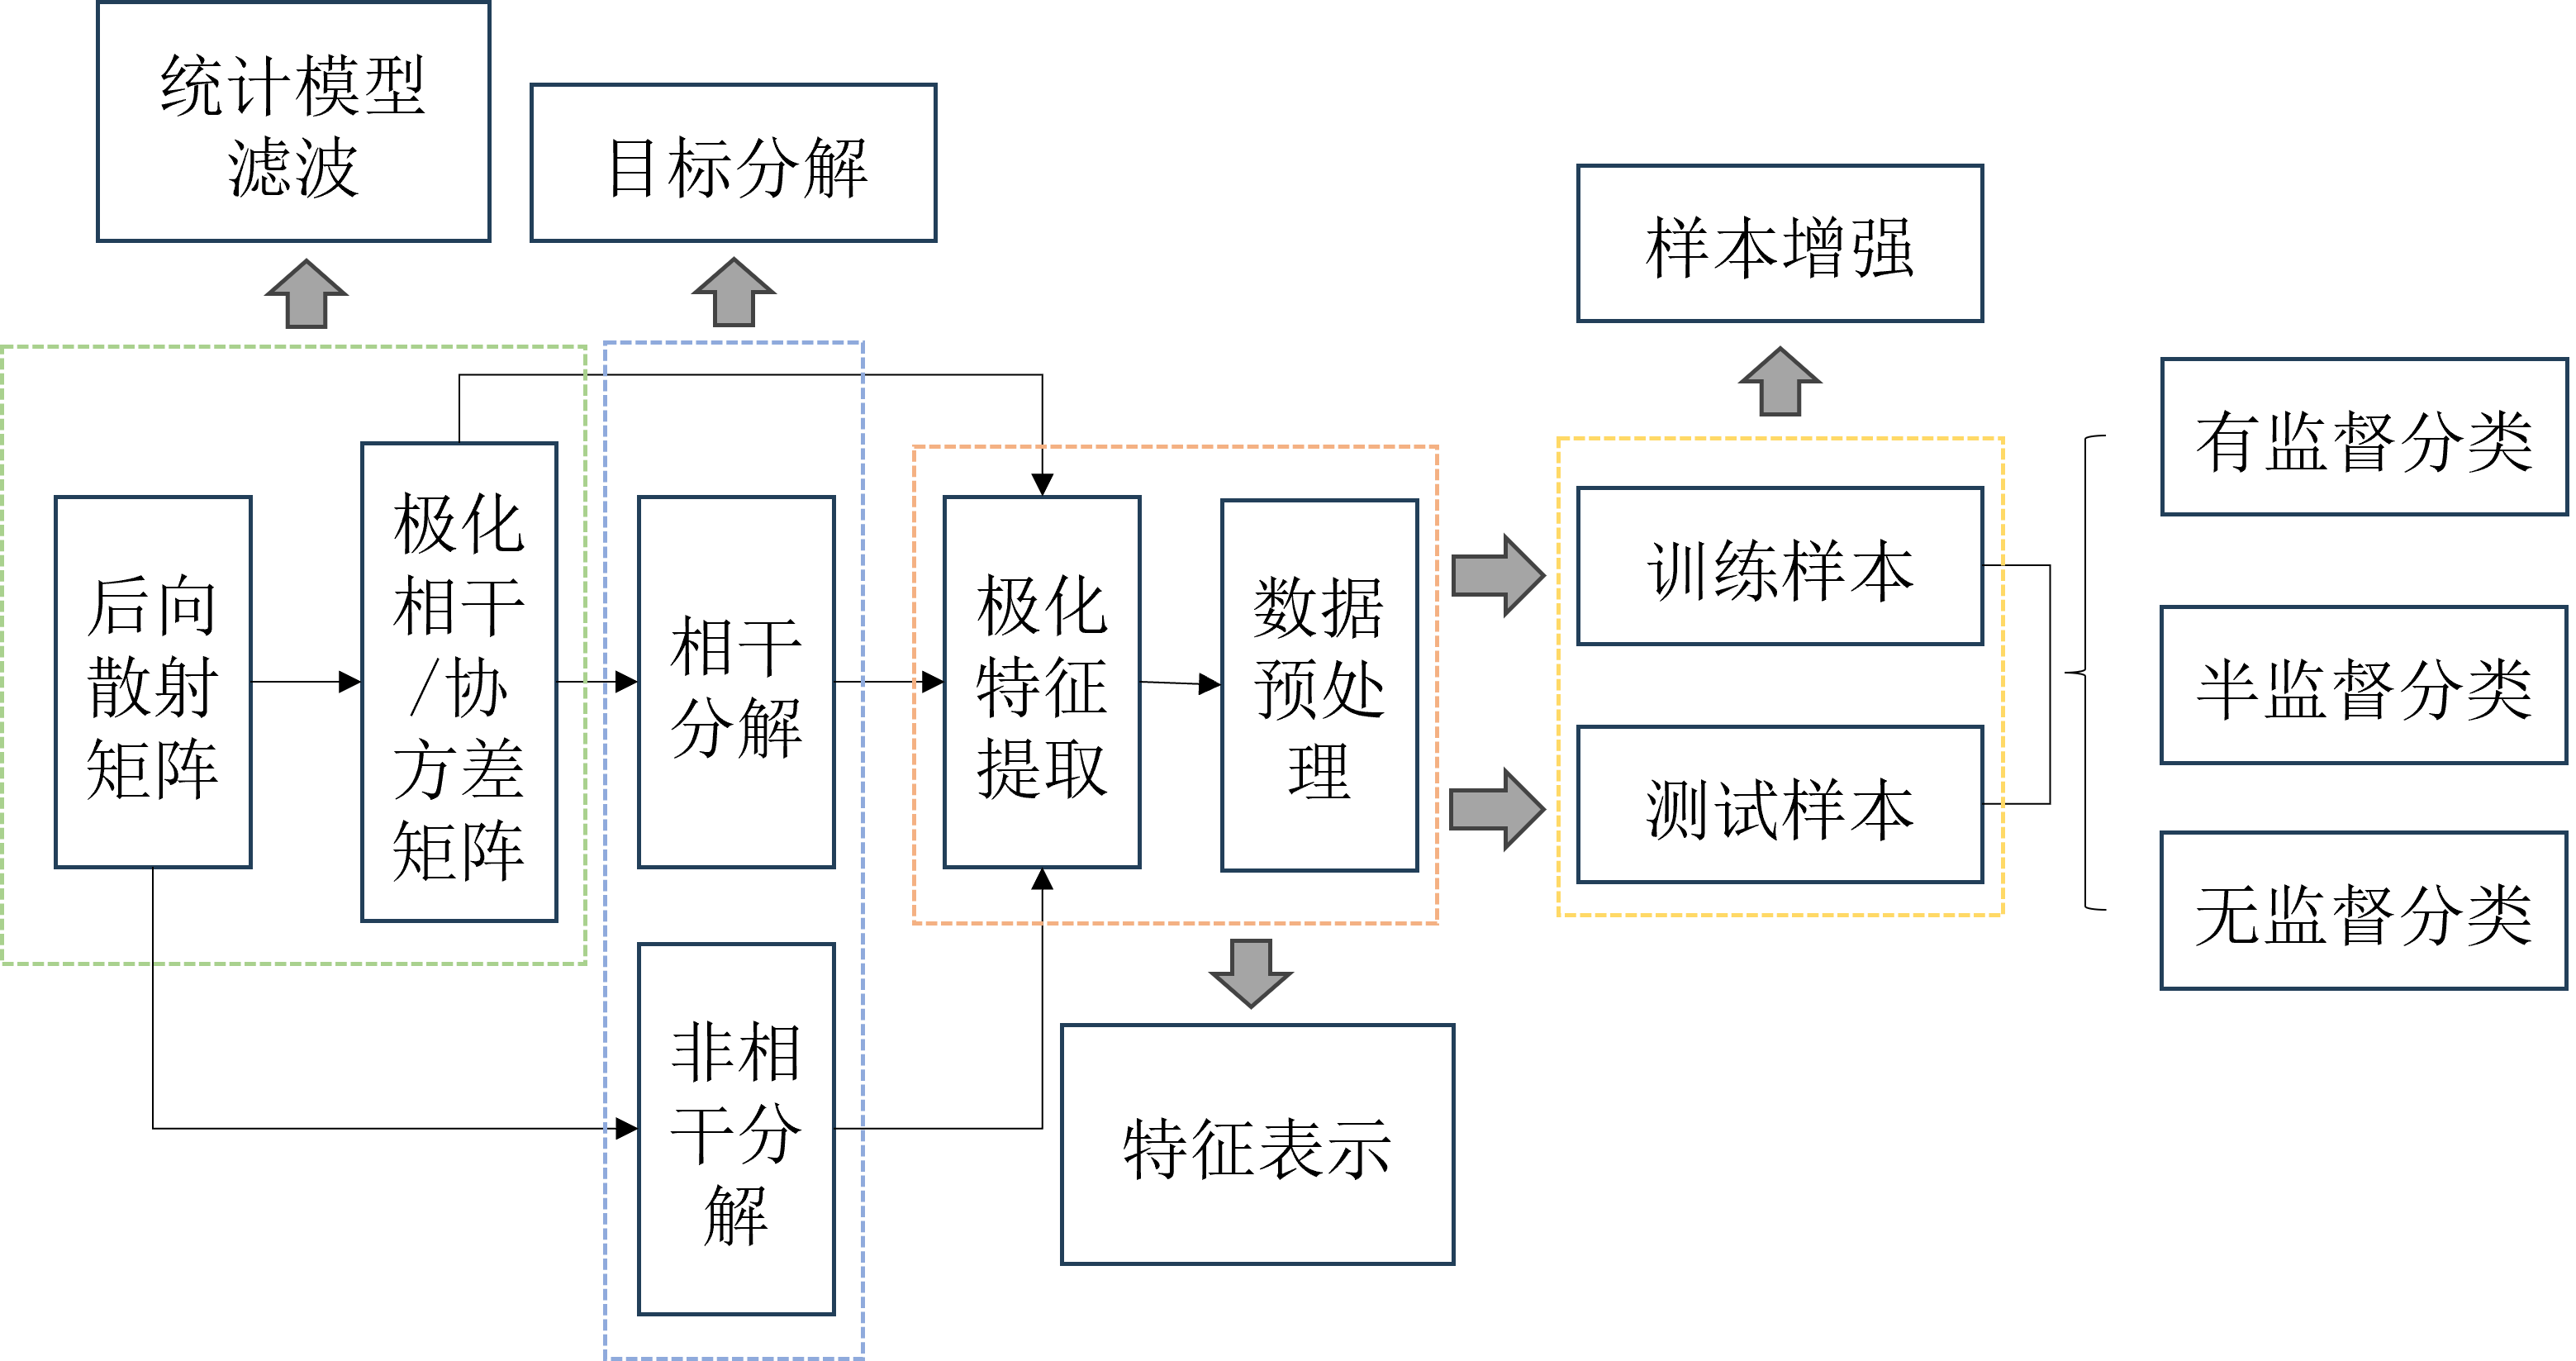
\includegraphics[width=12.3cm]{pic/chapter1/极化SAR分类流程.png}
  \caption{极化SAR图像目标分类流程}
  \label{fig:极化SAR图像目标分类流程}
\end{figure}


\subsubsection{无监督分类方法}
无监督极化SAR图像分类不需要预先存在的训练数据集。这类方法通常基于极化SAR图像本身的内在结构和特性,如散射机理分析、聚类算法(如K-means、谱聚类、密度峰聚类等)。这些方法试图发现图像数据内在的自然群体结构,根据极化散射特性的相似性将图像划分成不同的类别,但无法直接提供类别名称,而是生成潜在的集群划分。

Van Zyl等人\citing{van1989unsupervised}创新性地提出了基于入射和反射波相互作用关系的分类标准,首次将目标散射属性应用到分类方法;Cloude等人\citing{cloude1997entropy}提出了极化熵$\mathrm{H}$和平均散射角$\bar{\alpha}$的概念作为极化特征描述参数,并在$\mathrm{H}-\bar{\alpha}$二维空间划定了8个反映散射机制的区域,用于区分不同的目标类别;Lee等人\citing{lee1999unsupervised}在Cloude的研究成果上深化了无监督学习方法,开创性地结合了地物目标散射特性和统计特性,为后续无监督研究提供了重要理论支撑。

% Van Zyl等人\citing{van1989unsupervised}提出了基于入射、反射波之间关系的分类准则,并且首次将极化SAR的目标散射特性运用到目标分类方法中;Cloude等人\citing{cloude1997entropy}创新性地提出了极化熵$\mathrm{H}$以及平均散射角$\bar{\alpha}$的极化特征描述概念,并在$\mathrm{H}-\bar{\alpha}$平面中划分了8个代表不同散射机理的区域,来表示不同的地物类型;Lee等人\citing{lee1999unsupervised}在Cloude的研究基础上进一步提出了利用复Wishart分布的无监督学习方法,开创新地将地物目标物理散射特性和统计特征相结合,为后续的无监督研究工作提供了启发性的思路。

Ferro-Famil等人\citing{ferro2001unsupervised}在Cloude等人基础上进一步引入了各项异度性参数$\mathrm{A}$,并将$\mathrm{H}-\bar{\alpha}$图上的区域细分至16个,捕捉更多的细节信息,从而提高分类精度;Yamaguchi等人\citing{kimura2003pi}结合散射总功率SPAN设计了无监督分类方法,提高分类过程的收敛性;Lee等人\citing{lee2004unsupervised}在Freeman的研究基础上,整合了复Wishart分类方法,采用先模糊分类再精细化分类的粗略,通过迭代Wishart方法得到最终的分类结果。Bi等人\citing{bi2017polsar}提出了一种融合目标分解理论和K-Wishart似然分类的无监督分类方案,首先依据Pottier和Lee的方法生成初步的分类结果,继而利用多元极化特征及K-Wishart分类方法中的最大似然方法对结果进行精细分类,从而实现更高精度的分类效果。

% Ferro-Famil等人\citing{ferro2001unsupervised}引入了在Cloude的研究基础上引入了各项异度性$\mathrm{A}$,并且进一步地将$\mathrm{H}-\bar{\alpha}$的8区域扩展为16个区域,使分类结果更加准确,包含更多的细节;Yamaguchi等人\citing{kimura2003pi}将散射总功率SPAN与分类方法相结合,获得更好收敛性的无监督分类方法;Lee等人\citing{lee2004unsupervised}在Freeman分解的基础上,将基于复Wishart分类方法与Freeman分解相结合,通过先进行模糊分类,然后进行精细分类的方式,最后利用Wishart进行迭代分类得到最终的分类结果;Bi等人\citing{bi2017polsar}提出了一种基于目标分解理论和K-Wishart似然分类方法相结合的无监督分类方法,基于Pottier和Lee的方法先产生粗分类结果,然后利用多个不同的极化特征和K-Wishart分类方法的最大似然算法实现精确分类。

% 虽然无监督分类技术能够充分利用极化SAR数据的目标散射特性和统计分布特性,但由于缺乏标注样本,在处理同物异谱和异物同谱的情况时,往往无法达到理想的分类效果。

尽管无监督分类方法能够深入挖掘极化SAR数据所蕴含的目标统计分布规律和目标散射特性,但其在实践中受限于样本类别信息缺失,在面对同种物质表现出不同回波谱特性和不同物质却呈现相似回波谱特性的情形时,难以达到期望的分类性能。

\subsubsection{有监督分类方法}
相比于无监督分类方法,有监督的分类策略在指定分类规则过程中,得益于标记数据的辅助,能够进行更为精确的匹配训练,从而能够带来更为出色的分类结果。近年来,由于深度学习的自动挖掘数据鉴别特征和优越的分类性能,广泛的应用于自然语言处理、智能驾驶、信息检索等领域。由于其优越的性质,越来越多的研究将深度学习方法应用到遥感图像解译领域中,也获得了巨大的成果。

% 基于统计理论的分类方法是极化SAR图像分类领域应用最为广泛的方法,也被成为基于贝叶斯理论的分类方法。Kong等人\citing{1988Identification}从极化矢量服从高斯分布这一特性出发,构建了基于复高斯分布的最大似然分类器;Lee等人\citing{lee1999unsupervised,lee1994classification}利用相干矩阵服从Wishart分布理论基础,提出了Wishart分类器。

% 除了以上提及的基于极化SAR数据分布特性的有监督分类方法,

Lv等人\citing{lv2014classification}将深度信念网络(Deep Belief Network, DBN)应用到极化SAR图像分类中,并取得了优异的分类效果;Xie等人\citing{xie2014multilayer}利用堆叠式自编码器(Stacked Sparse Autoencoder, SSAE)来获取可鉴别特征,随后基于标签微调,实现了分类性能和区域分类视觉效果上的巨大提升。Zhou等人\citing{zhou2016polarimetric}使用一维向量来表征极化SAR数据的相干矩阵,并将其作为CNN的输入作为分类,开创性地将卷积网络分类方法引入到极化SAR图像分类中。Zhang等人\citing{zhang2017complex}构建了一种复数卷积网络结构(Complex-valued CNN, CV-CNN),该模型将传统卷积网络中的核心组成模块——卷积层、池化层、激活函数以及全连接层等均推广至复数形式,还提出了一种专为复数域设计的反向传播优化策略,为后续的一系列设计复数域的分类算法奠定了技术基础。


% Zhang等人\citing{zhang2017complex}在Zhou的研究基础上提出了基于复数的卷积网络结构(Complex-valued CNN, CV-CNN),通过将卷积网络中的基本模块,包括卷积层、池化层、激活函数、全连接层等均扩展至复数的形式,并且提出了适用于复数域的反向传播优化算法,进一步提升了CNN在极化SAR图像分类任务中的分类准确率,并且为后续的一系列复数域分类算法奠定了基础。

\subsubsection{半监督分类方法}
半监督分类方法旨在结合监督学习和无监督学习方法,同时利用有标签样本数据和无标签样本数据对分类模型进行训练。实际场景中,要获取充足数量的高质量训练样本通常是非常困难的,深度网络训练过程仅有少量标记样本和大量无标记样本。因此,如何利用大量的无标签数据和少量的标记样本来辅助网络学习到更加准确的分类规则,已经成为一个研究重点。

Liu等人\citing{liu2016large}采用图构建技术,通过选取特定的锚点来构造邻接矩阵,旨在实现从有限标签样本到大规模无标签样本的信息扩散过程;Hou等人\citing{hou2017robust}基于字典学习和区域一致特性,学习到稀疏的高级特征之后结合无标签样本实现分类器的训练;Jie等人\citing{geng2017semisupervised}基于超像素方法来应对极化SAR中存在的相干斑噪声的问题;Liu等人\citing{liu2018fully}和Liu等人\citing{liu2019task}利用无标签样本数据,通过生成对抗网络学习到数据的分布特性,实现生成样本扩充训练集数量。

% Liu等人\citing{liu2016large}通过建图的方法,利用选定的锚点来构建邻接矩阵,实现从有标签样本到无标签样本的标签传播;

以上所提及的代表性方法均在极化SAR图像分类中取得了显著的成果,有效推动了极化SAR目标分类的研究。但目前主流研究广泛采用散射矩阵或相干矩阵作为网络输入,尚未充分挖掘和利用极化SAR图像数据内在的多类型极化特征所蕴含的全部信息,如何利用深度网络来探索有效的极化特征信息表示方式仍然需要进一步的研究。此外,现有极化SAR图像分类研究大多在理想的高质量、数量充足的训练集条件下完成,而针对训练样本中存在错误标记的标签噪声样本缺乏考虑,如何在混杂有噪声样本的数据集下实现高准确率的分类结果也需要进一步展开研究。

\section{论文主要内容及章节安排}
针对极化SAR多类型极化特征信息冗余与标签噪声下目标分类问题,本文从极化SAR相关理论基础、多类型极化信息利用以及标签噪声下目标分类方法三个方面展开研究。本文共分为五个章节,各章节结构安排为:

第一章:绪论。阐述本文工作的研究背景与意义,并且对其中的极化特征表示、极化SAR目标分类方法进行国内外研究现状进行概括分析,最后给出全文的结构安排。

第二章:介绍极化SAR相关理论基础。首先,介绍了电磁波的极化特性及其数学表征方式。其次,介绍了针对目标散射特性的极化散射矩阵和二阶统计矩阵两种描述方法。最后,介绍了极化相干与非相干目标分解方法,并总结归纳了不同极化参数的物理含义,为本文的研究工作奠定理论基础。

第三章:介绍所提出的双通道注意力的极化SAR目标分类方法。首先,简要阐述多类型极化特征利用存在的相关问题。其次,分别介绍了通道、空间以及混合注意力方法的基础原理。随后,介绍提出的双通道注意力的极化SAR目标分类方法,并对方法中的模块细节、原理设计进行了相关阐述。最后,基于真实极化SAR数据集进行验证测试,根据实验结果从视觉和数值方面对提出方法性能进行评价。

% 第三章:针对极化SAR多类型特征信息冗余问题,提出了一种基于双通道注意力的极化SAR目标分类方法。该方法利用后向散射信息与极化目标分解信息之间的差异性与互补性,通过双通道的网络结构形式,对两种类型的极化信息进行充分细化和有效融合。同时,增加了跨空间学习方法,有效地聚合不同尺寸的极化特征,充分利用空间尺寸层次的极化信息。最后,利用两组真实极化SAR数据对该方法进行有效性验证,实验结果表明该方法能为极化SAR数据提供更加全面、充分的表达方式,实现极化SAR图像更加精确的分类结果。

第四章:介绍所提出的标签噪声下鲁棒性的极化SAR目标分类方法。首先,简要阐述极化SAR图像解译中存在的标签噪声问题及其为目标分类任务带来的影响。其次,简要介绍了有限混合模型基本原理,并分析了不同混合模型的优缺点。随后,重点叙述了所提出的基于混合模型与边界增强的极化SAR目标分类方法,介绍了混合模型概率估计原理以及边界增强模块详细执行步骤,并导出分类模型鲁棒损失优化函数。最后,基于真实极化SAR数据集对不同标签噪声源进行验证测试,根据实验结果从视觉和数值方面对提出方法性能进行评价。


% 第四章:针对极化SAR分类中的标签噪声问题,提出了一种基于混合模型与边界增强的极化SAR目标分类方法。该方法首先利用噪声、干净样本在深度网络模型中损失的分布差异性,基于贝塔混合模型对损失分布进行建模,实现样本噪声概率估计。同时,为了增强模型对边界信息的利用,基于Sobel算子对Pauli图像进行边界提取并膨胀,对膨胀边界内的样本增加额外的损失惩罚。在此基础上,改进自学习损失函数,通过样本噪声概率估计对预测项和真值标签的动态调整,实现鲁棒的训练过程。最后,结合极化信息提取器,利用两组真实极化SAR数据对该方法进行有效性验证,实验结果表明本章方法对不同噪声源均具有良好的鲁棒性能。

第五章:对本文研究工作进行总结,并展望未来工作。